\chapter{ĐIỀU KHIỂN VÀ LẬP TRÌNH}
\section{Tổng quan về phần điều khiển}
\subsection{Sơ đồ khối hệ thống điều khiển}
\begin{figure}[htp]
	\centering
	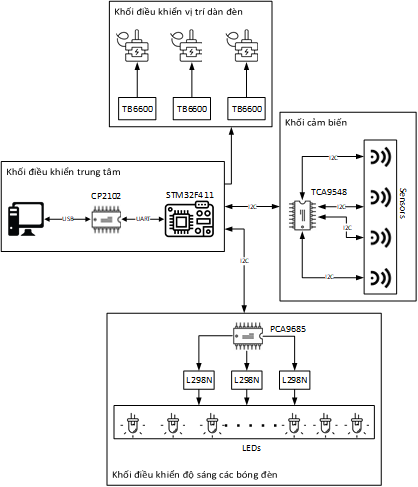
\includegraphics[scale=1]{Chapters/Chapter5/Images/Sodokhoihethong.png}
	\caption{Sơ đồ khối hệ thống điều khiển}
	\label{fig:C5Sodokhoihethong}
\end{figure}

\subsection{Khối điều khiển trung tâm}
\begin{itemize}
\item PC: dùng 1 phần mềm giao diện để gửi tín hiệu điều khiển xuống VĐK và hiển thị dữ liệu do VĐK trả về.
\item VĐK STM32F4: thực hiện các tác vụ chính của hệ thống: truyền nhận tín hiệu I2C với các module, xuất tín hiệu logic tới driver động cơ bước.
\item Module USB to UART CP2102: chuyển đổi giao tiếp từ USB để PC và VĐK có thể giao tiếp với nhau qua chuẩn giao tiếp UART.
\end{itemize}
\begin{figure}[htp]
	\centering
	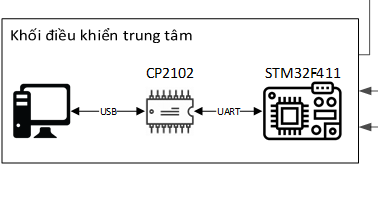
\includegraphics[scale=1]{Chapters/Chapter5/Images/Khoidieukhientrungtam.png}
	\caption{Khối điều khiển trung tâm}
	\label{fig:C5central}
\end{figure}

\subsection{Khối cảm biến}
\begin{figure}[htp]
	\centering
	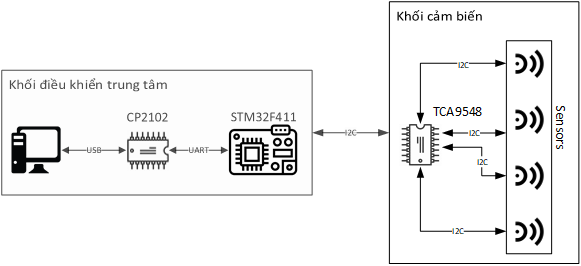
\includegraphics[scale=1]{Chapters/Chapter5/Images/KhoiSensor.png}
	\caption{Khối cảm biến}
	\label{fig:C5Sensor}
\end{figure}
\begin{itemize}
\item Module TCA9548: mở rộng kênh I2C, khuếch đại tín hiệu trên 2 đường dẫn SCL và SDA.
\item Sensors: các module cảm biến GY-30 BH1750. Đo lường cường độ ánh sáng và gửi về VĐK bằng chuẩn giao tiếp I2C.
\end{itemize}

\subsection{Khối điều khiển vị trí các dàn đèn}
\begin{figure}[htp]
	\centering
	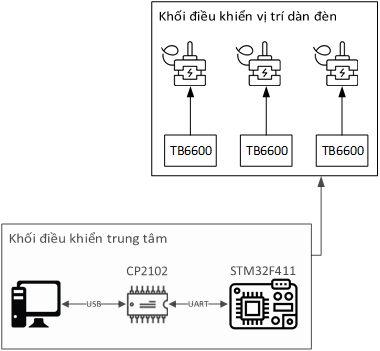
\includegraphics[scale=1]{Chapters/Chapter5/Images/Khoidieukhienlocation.png}
	\caption{Khối điều khiển vị trí các dàn đèn}
	\label{fig:C5Khoidieukhienvitridanden}
\end{figure}
\begin{itemize}
\item Các module TB6600: Nhận xung điều khiển từ VĐK và điều khiển các động cơ quay theo xung điều khiển.
\item Động cơ bước: thông qua bộ truyền đai kéo các dàn đèn để điều khiển dàn đèn tới vị trí mong muốn.
\end{itemize}

\subsection{Khối điều khiển độ sáng các bóng đèn}
\begin{figure}[htp]
	\centering
	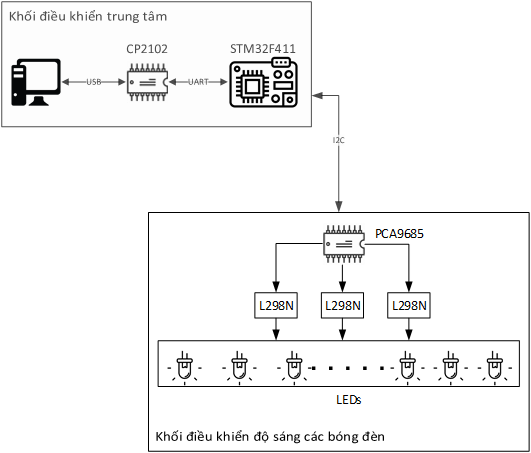
\includegraphics[scale=1]{Chapters/Chapter5/Images/KhoidieukhienLED.png}
	\caption{Khối điều khiển độ sáng các bóng đèn}
	\label{fig:C5KhoidieukhienLED}
\end{figure}
\begin{itemize}
\item PCA9685: Xuất xung PWM để điều khiển độ sáng các bóng đèn.
\item L298N: Nhận xung PWM từ PCA9685 để điều khiển độ sáng bóng đèn lấy nguồn từ bộ nguồn 12V.
\item Bóng đèn LED: Chiếu sáng cho mô hình.
\end{itemize}
\clearpage

\section{Lập trình các chức năng Manual}
\subsection{Lưu đồ giải thuật chương trình điều khiển}
\begin{figure}[H]
	\centering
	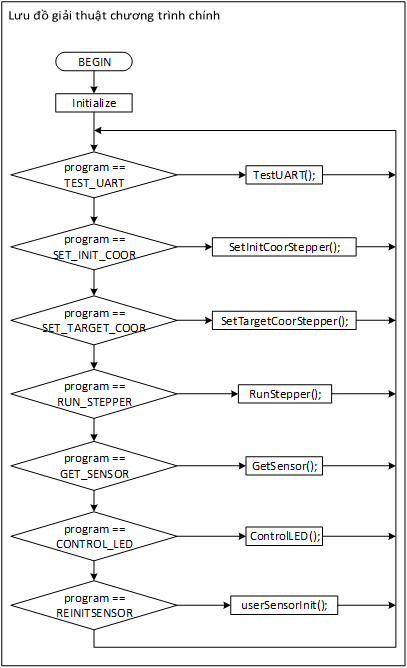
\includegraphics[scale=1]{Chapters/Chapter5/Images/Luudogiaithuatmain.png}
	\caption{Lưu đồ giải thuật chương trình chính}
	\label{fig:C5main}
\end{figure}
\begin{figure}[ht]
	\centering
	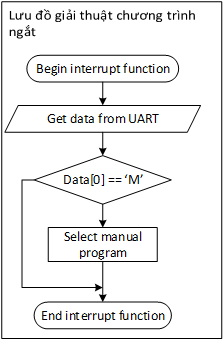
\includegraphics[scale=1]{Chapters/Chapter5/Images/Luudogiaithuatinterrupt.png}
	\caption{Lưu đồ giải thuật chương trình ngắt}
	\label{fig:C5interrupt}
\end{figure}

\subsection{Đọc dữ liệu từ cảm biến}
Một cảm biến ánh sáng GY-30 BH1750 chỉ có thể cài đặt được 2 địa chỉ I2C là “1011100” (0x5C) và “0100011” (0x23). Như vậy 1 kênh I2C chỉ có thể kết nối được tối đa 2 cảm biến. Vi điều khiển STM32F411VETx chỉ có 3 kênh I2C trong khi số cảm biến cần kết nối rất nhiều (16 cảm biến), nên nhóm dùng thêm module tăng số kênh I2C TCA9548A, mở rộng từ 1 kênh I2C lên 8 kênh I2C.

Nhà sản xuất chỉ có sẵn thư viện cho BH1750 và TCA9548A cho dòng VDK  Atmega328P. Vì thế, nhóm phải tự viết lại thư viện riêng dùng bộ thư viện HAL cho dòng VDK STM32F4.

\textbf{Module TCA9548A:}

\textbf{\textit{Địa chỉ I2C:}}
\begin{figure}[H]
	\centering
	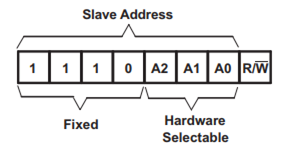
\includegraphics[scale=1]{Chapters/Chapter5/Images/AddressTCA}
	\caption{Địa chỉ I2C của module TCA9548A}
	\label{fig:C5AddressTCA}
\end{figure}

Khi 3 chân A0, A1, A2 trên module được thả nổi thì module sẽ có địa chỉ I2C là 0b1110000 hay 0x70.

\textbf{\textit{Gửi data cho module:}}
\begin{figure}[H]
	\centering
	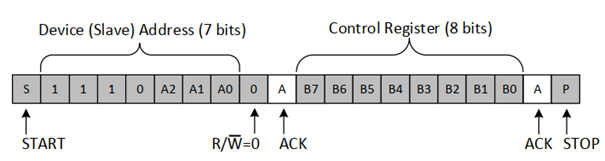
\includegraphics[scale=0.9]{Chapters/Chapter5/Images/SendDataTCA.png}
	\caption{Quy cách gửi data cho module TCA9548A}
	\label{fig:C5SendDataTCA}
\end{figure}

\textbf{\textit{Đọc dữ liệu từ module:}}
\begin{figure}[H]
	\centering
	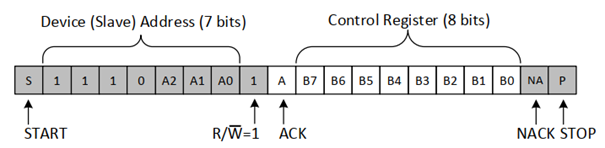
\includegraphics[scale=0.9]{Chapters/Chapter5/Images/ReadDataTCA.png}
	\caption{Quy cách đọc data từ module TCA9548A}
	\label{fig:C5ReadDataTCA}
\end{figure}

\textbf{\textit{Bảng định nghĩa hàm dựa trên control register:}}
\begin{figure}[H]
	\centering
	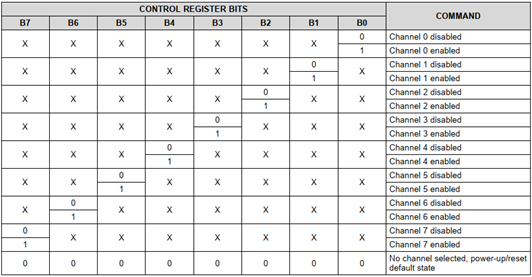
\includegraphics[scale=1]{Chapters/Chapter5/Images/ControlRegisterTCA.png}
	\caption{Bảng định nghĩa hàm dựa trên Control Register của TCA9548A}
	\label{fig:C5ControlRegisterTCA}
\end{figure}

\textbf{Thư viện cho module TCA9548A}
\begin{lstlisting}
\\ TCA9548A_Driver.h
#ifndef TCA9548_H_
#define TCA9548_H_

#include "main.h"
#include "stm32f4xx_hal_i2c.h"

#define TCA_ADDRESS (0x70 << 1)

typedef enum {
    TCA9548A_OK = 0,
    TCA9548A_ERROR = 1
} TCA9548A_STATUS;

typedef struct TCA9548_Driver {
    I2C_HandleTypeDef *I2C_channel;
    uint8_t Address;
} TCA9548A_HandleTypeDef;

TCA9548A_STATUS TCA9548A_Init(TCA9548A_HandleTypeDef *htca9548a, I2C_HandleTypeDef *hi2c, uint16_t address);
TCA9548A_STATUS TCA9548A_SelectSingleChannel(TCA9548A_HandleTypeDef *htca9548a, uint8_t channel);
TCA9548A_STATUS TCA9548A_SelectMultiChannel(TCA9548A_HandleTypeDef *htca9548a, uint8_t channel);
uint8_t TCA9548A_ReadStatus(TCA9548A_HandleTypeDef *htca9548a);
TCA9548A_STATUS TCA9548A_DisableAllChannel(TCA9548A_HandleTypeDef *htca9548a);

#endif
\end{lstlisting}

\begin{lstlisting}
\\ TCA9548A_Driver.c
#include "TCA9548A_Driver.h"

/*
 * @brief Initialize
 * @param htca9548a Pointer to a TCA9548A_HandleTypeDef
 * @param hi2c Pointer to a I2C_HandleTypeDef structure that contains
 *               the configuration information for the specified I2C.
 * @param address Target BH1750 device address. The device 7 bits address value in datasheet must
 *                be shifted to the left before calling by I2C function.
 * @retval TCA9548A Status
 */
TCA9548A_STATUS TCA9548A_Init(TCA9548A_HandleTypeDef *htca9548a, I2C_HandleTypeDef *hi2c, uint16_t address) {
    htca9548a->I2C_channel = hi2c;
    htca9548a->Address = address;

    if (TCA9548A_OK == TCA9548A_DisableAllChannel(htca9548a)) {
        return TCA9548A_OK;
    }
    return TCA9548A_ERROR;
}

/*
 * @brief Initialize
 * @param htca9548a Pointer to a TCA9548A_HandleTypeDef
 * @param channel From 0 to 7, is channel 0 to channel 7 on TCA9548A
 * @retval TCA9548A Status
 */
TCA9548A_STATUS TCA9548A_SelectSingleChannel(TCA9548A_HandleTypeDef *htca9548a, uint8_t channel) {
    if (channel > 7) {
        return TCA9548A_ERROR;
    }
    uint8_t tmp = (1 << channel);
    if (HAL_OK == HAL_I2C_Master_Transmit(htca9548a->I2C_channel, htca9548a->Address, &tmp, 1, 10)) {
        return TCA9548A_OK;
    }
    return TCA9548A_ERROR;
}

/*
 * @brief Initialize
 * @param htca9548a Pointer to a TCA9548A_HandleTypeDef
 * @param channel This have 8 bit to choose which channel is selected.
 *                Ex: channel 0, 3, 5 is selected, channel = 0b00101001 = 0x29 
 * @retval TCA9548A Status
 */
TCA9548A_STATUS TCA9548A_SelectMultiChannel(TCA9548A_HandleTypeDef *htca9548a, uint8_t channel) {
    if (HAL_OK == HAL_I2C_Master_Transmit(htca9548a->I2C_channel, htca9548a->Address, &channel, 1, 10)) {
        return TCA9548A_OK;
    }
    return TCA9548A_ERROR;
}

uint8_t TCA9548A_ReadStatus(TCA9548A_HandleTypeDef *htca9548a) {
    uint8_t tmp;
    if (HAL_OK == HAL_I2C_Master_Receive(htca9548a->I2C_channel, htca9548a->Address, &tmp, 1, 10)) {
        return tmp;
    }
    return 0;
}

TCA9548A_STATUS TCA9548A_DisableAllChannel(TCA9548A_HandleTypeDef *htca9548a) {
    uint8_t tmp = 0x00;
    if (HAL_OK == HAL_I2C_Master_Transmit(htca9548a->I2C_channel, htca9548a->Address, &tmp, 1, 10)) {
        return TCA9548A_OK;
    }
    return TCA9548A_ERROR;
}
\end{lstlisting}
\clearpage

\textbf{Module GY-30 BH1750}

\textbf{\textit{Địa chỉ I2C}}

Khi chân ADDR của module có tín hiệu mức cao $(\geq 0.7VCC)$ thì module có địa chỉ là: 0b1011100 hay 0x5C, ngược lại module sẽ có địa chỉ là 0b0100011 hay 0x23.

\textbf{\textit{Gửi data cho module:}}
\begin{figure}[H]
	\centering
	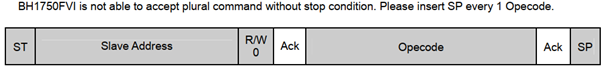
\includegraphics[scale=0.9]{Chapters/Chapter5/Images/SendDataGY30.png}
	\caption{Gửi data cho module BH1750}
	\label{fig:C5SendDataGY30}
\end{figure}

\textbf{\textit{Đọc data từ module:}}
\begin{figure}[H]
	\centering
	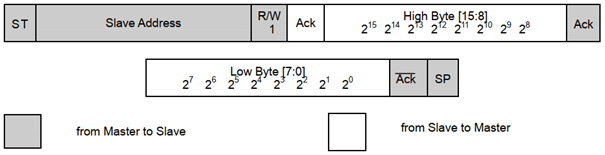
\includegraphics[scale=0.9]{Chapters/Chapter5/Images/ReadDataGY30.png}
	\caption{Đọc data từ module BH1750}
	\label{fig:C5ReadDataGY30}
\end{figure}

\textbf{\textit{Bảng mã điều khiển:}}
\begin{figure}[H]
	\centering
	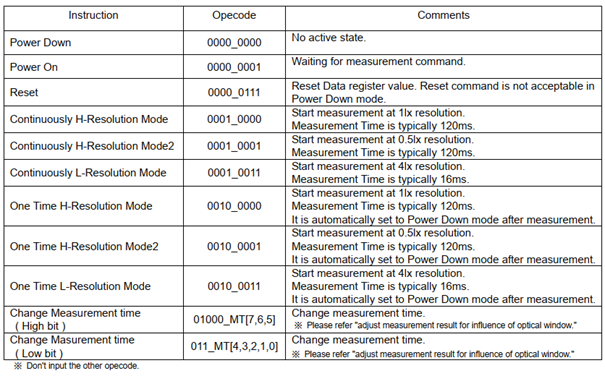
\includegraphics[scale=0.9]{Chapters/Chapter5/Images/OpecodeGY30.png}
	\caption{Bảng mã điều khiển của module BH1750}
	\label{fig:C5OpecodeGY30}
\end{figure}

\textbf{Thư viện cho module GY-30 BH1750:}
\begin{lstlisting}
\\ BH1750_Driver.h
#ifndef BH1750_H_
#define BH1750_H_

/* Include ------------ */
#include "stm32f4xx_hal.h"

#define BH1750_ADDRESS_HIGH        (0x5C<<1)
#define BH1750_ADDRESS_LOW         (0x23<<1)

#define BH1750_POWER_DOWN          0x00
#define BH1750_POWER_ON            0x01
#define BH1750_RESET               0x07

#define BH1750_DEFAULT_MTREG       69
#define BH1750_CONVERSION_FACTOR   1.2

typedef enum {
    BH1750_OK    = 0,
    BH1750_ERROR = 1
} BH1750_STATUS;

typedef enum {
    CONTINUOUS_H_RES_MODE    = 0x10,
    CONTINUOUS_H_RES_MODE2   = 0x11,
    CONTINUOUS_L_RES_MODE    = 0x13,
    ONETIME_H_RES_MODE       = 0x20,
    ONETIME_H_RES_MODE2      = 0x21,
    ONETIME_L_RES_MODE       = 0x23
} bh1750_mode;

typedef struct BH1750_Driver
{
    I2C_HandleTypeDef *I2C_channel;
    uint16_t Address;

} BH1750_HandleTypeDef;

BH1750_STATUS BH1750_Init(BH1750_HandleTypeDef *hbh1750, I2C_HandleTypeDef *hi2c, uint16_t Address);
BH1750_STATUS BH1750_Reset(BH1750_HandleTypeDef *hbh1750);
BH1750_STATUS BH1750_PowerState(BH1750_HandleTypeDef *hbh1750, uint8_t PowerOn);
BH1750_STATUS BH1750_SetMtreg(BH1750_HandleTypeDef *hbh1750, uint8_t Mtreg);
BH1750_STATUS BH1750_SetMode(BH1750_HandleTypeDef *hbh1750, bh1750_mode Mode);
BH1750_STATUS BH1750_TriggerManualConversion(BH1750_HandleTypeDef *hbh1750);
BH1750_STATUS BH1750_ReadLight(BH1750_HandleTypeDef *hbh1750, uint16_t *Result);

#endif /* BH1750_H_ */
\end{lstlisting}

\begin{lstlisting}
\\ BH1750_Driver.c
/*
 =======================================================
          ##### How to use this driver #####
 =======================================================
    Set up:
    #1  @ref BH1750_Init()
        Ex: BH1750_Init(&sensor[i], &hi2c1, BH1750_ADDRESS_LOW);
    #2  @ref BH1750_PowerState()
        Ex: BH1750_PowerState(&sensor[i], 1);
    #3  @ref BH1750_SetMode()
        Ex: BH1750_SetMode(&sensor[i], CONTINUOUS_H_RES_MODE);
        
    Let play: Read light @ref BH1750_ReadLight()
    BH1750_ReadLight(&sensor[i], &result[i]);
*/

#include "BH1750_Driver.h"

bh1750_mode     BH1750_Mode;
uint8_t         BH1750_Mtreg;

/*
 * @brief Initialize
 * @param hbh1750 Pointer to a BH1750_HandleTypeDef
 * @param hi2c Pointer to a I2C_HandleTypeDef structure that contains
 *               the configuration information for the specified I2C.
 * @param Address Target BH1750 device address. The device 7 bits address value in datasheet must
 *                be shifted to the left before calling by I2C function.
 * @retval BH1750 Status
 */
BH1750_STATUS BH1750_Init(BH1750_HandleTypeDef *hbh1750, I2C_HandleTypeDef *hi2c, uint16_t Address) {
    hbh1750->I2C_channel = hi2c;
    hbh1750->Address = Address;
    if(BH1750_OK == BH1750_Reset(hbh1750))
    {
        if(BH1750_OK == BH1750_SetMtreg(hbh1750, BH1750_DEFAULT_MTREG)) // Set default value;
            return BH1750_OK;
    }
    return BH1750_ERROR;
}

/* 
 * @brief Reset all registers to default value.
 * @param hbh1750 Pointer to a BH1750_HandleTypeDef
 * @retval BH1750 status
 */
BH1750_STATUS BH1750_Reset(BH1750_HandleTypeDef *hbh1750) {
    uint8_t tmp = BH1750_RESET;
    if (HAL_OK == HAL_I2C_Master_Transmit(hbh1750->I2C_channel, hbh1750->Address, &tmp, 1, 10))
        return BH1750_OK;
    return BH1750_ERROR;
}

/*
 * @brief Set the power state.
 * @param hbh1750 Pointer to a BH1750_HandleTypeDef
 * @param PowerOn
 *          @arg 0: Power down, low current, no active state.
 *          @arg 1: Ready for measurement command. 
 * @retval BH1750 status
 */
BH1750_STATUS BH1750_PowerState(BH1750_HandleTypeDef *hbh1750, uint8_t PowerOn) {
    PowerOn = (PowerOn ? 1 : 0);
    if (HAL_OK == HAL_I2C_Master_Transmit(hbh1750->I2C_channel, hbh1750->Address, &PowerOn, 1, 10))
        return BH1750_OK;
    return BH1750_ERROR;
}

/*
 * @brief Adjust measurement result for influence of optical window. (sensor sensitivity adjusting) 
 * @param hbh1750 Pointer to a BH1750_HandleTypeDef
 * @param Mtreg The modified value of measurement time register. (31 <= Mtreg <=254) (miliseconds)
 * @retval BH1750 status
 */
BH1750_STATUS BH1750_SetMtreg(BH1750_HandleTypeDef *hbh1750, uint8_t Mtreg) {
    HAL_StatusTypeDef retCode;
    if (Mtreg < 31 || Mtreg > 254) {
        return BH1750_ERROR;
    }

    BH1750_Mtreg = Mtreg;

    uint8_t tmp[2];

    tmp[0] = (0x40 | (Mtreg >> 5));     // High bit 01000_MT[7,6,5]
    tmp[1] = (0x60 | (Mtreg & 0x1F));   // Low bit  011_MT[4,3,2,1,0] 

    retCode = HAL_I2C_Master_Transmit(hbh1750->I2C_channel, hbh1750->Address, &tmp[0], 1, 10);
    if (HAL_OK != retCode) {
        return BH1750_ERROR;
    }

    retCode = HAL_I2C_Master_Transmit(hbh1750->I2C_channel, hbh1750->Address, &tmp[1], 1, 10);
    if (HAL_OK == retCode) {
        return BH1750_OK;
    }

    return BH1750_ERROR;
}

/*
 * @brief Set the mode of converting. Look into bh1750_mode enum.
 * @param hbh1750 Pointer to a BH1750_HandleTypeDef
 * @param Mode The mode of converting. This parameter can be one of the bh1750_mode enum values:
 *              @arg CONTINUOUS_H_RES_MODE:  Start measurement at 1lx resolution.
 *                                           Measurement Time is typically 120ms. 
 *              @arg CONTINUOUS_H_RES_MODE2: Start measurement at 0.5lx resolution.
 *                                           Measurement Time is typically 120ms. 
 *              @arg CONTINUOUS_L_RES_MODE:  Start measurement at 4lx resolution. 
 *                                           Measurement Time is typically 16ms. 
 *              @arg ONETIME_H_RES_MODE:     Start measurement at 1lx resolution.
 *                                           Measurement Time is typically 120ms. 
 *                                           It is automatically set to Power Down mode after measurement.
 *              @arg ONETIME_H_RES_MODE2:    Start measurement at 0.5lx resolution.
 *                                           Measurement Time is typically 120ms. 
 *                                           It is automatically set to Power Down mode after measurement.
 *              @arg ONETIME_L_RES_MODE:     Start measurement at 4lx resolution.
 *                                           Measurement Time is typically 16ms. 
 *                                           It is automatically set to Power Down mode after measurement.
 * @retval BH1750 status
 */
BH1750_STATUS BH1750_SetMode(BH1750_HandleTypeDef *hbh1750, bh1750_mode Mode) {
    if(!((Mode >> 4) || (Mode >> 5))) return BH1750_ERROR;
    if((Mode & 0x0F) > 3) return BH1750_ERROR;

    BH1750_Mode = Mode;
    if(HAL_OK == HAL_I2C_Master_Transmit(hbh1750->I2C_channel, hbh1750->Address, &Mode, 1, 10))
        return BH1750_OK;

    return BH1750_ERROR;
}

// BH1750_STATUS BH1750_TriggerManualConversion(uint16_t Address);

/*
 * @brief Read the converted value and calculate the result.
 * @param hbh1750 Pointer to a BH1750_HandleTypeDef
 * @param Result Pointer to your variable for getting result.
 * @retval BH1750 Status
 */
BH1750_STATUS BH1750_ReadLight(BH1750_HandleTypeDef *hbh1750, uint16_t *Result) {
    uint16_t result;
    uint8_t tmp[2];

    if(HAL_OK == HAL_I2C_Master_Receive(hbh1750->I2C_channel, hbh1750->Address, tmp, 2, 10))
    {
        result = (tmp[0] << 8) | (tmp[1]);

        if(BH1750_Mtreg != BH1750_DEFAULT_MTREG)
        {
            result *= (float)((uint8_t)(BH1750_DEFAULT_MTREG) / (float)BH1750_Mtreg);
        }

        if(BH1750_Mode == ONETIME_H_RES_MODE2 || BH1750_Mode == CONTINUOUS_H_RES_MODE2)
        {
            result /= 2.0;
        }

        *Result = result / (float)BH1750_CONVERSION_FACTOR;
        return BH1750_OK;
    }
    return BH1750_ERROR;
}
\end{lstlisting}



Phần chương trình đọc dữ liệu cảm biến trong file main.c:
\begin{lstlisting}
// Variables for Sensor and TCA
TCA9548A_HandleTypeDef i2cHub;
BH1750_HandleTypeDef sensor[4];
char dataSensorMessage[24] = {};
uint16_t dataSensor[4];
uint8_t ret;
void userSensorInit() {
  TCA9548A_Init(&i2cHub, &hi2c1, TCA_ADDRESS);
  for (uint8_t i = 0; i < 4; i++) {
    TCA9548A_SelectSingleChannel(&i2cHub, i);
    BH1750_Init(&sensor[i], &hi2c1, BH1750_ADDRESS_LOW);
    BH1750_PowerState(&sensor[i], 1);
    BH1750_SetMode(&sensor[i], CONTINUOUS_H_RES_MODE);
  }
}
void GetSensor() {
  for (uint8_t i = 0; i < 4; i++) {
    TCA9548A_SelectSingleChannel(&i2cHub, i);
    BH1750_ReadLight(&sensor[i], &dataSensor[i]);

    dataSensorMessage[i*6 + 5] = (i < 3) ? ' ' : '\n';
    dataSensorMessage[i*6 + 4] = dataSensor[i] % 10 + '0';
    dataSensorMessage[i*6 + 3] = dataSensor[i] / 10 % 10 + '0';
    dataSensorMessage[i*6 + 2] = dataSensor[i] / 100 % 10 + '0';
    dataSensorMessage[i*6 + 1] = dataSensor[i] / 1000 % 10 + '0';
    dataSensorMessage[i*6 + 0] = dataSensor[i] / 10000 % 10 + '0';
  }
  HAL_UART_Transmit(&huart2, (uint8_t *)dataSensorMessage, 24, 24);
  program = IDLE;
}
\end{lstlisting}

\subsection{Điều khiển toạ độ các dàn đèn}
Tọa độ của các dàn đèn được điều khiển bởi các động cơ bước sử dụng TB6600 làm driver. 

\textbf{Thư viện cho Driver TB6600:}
\begin{lstlisting}
\\ Stepper_Driver.h
#ifndef STEPPERDRIVER_H_
#define STEPPERDRIVER_H_

#include "stm32f4xx_hal.h"

// Time delay write HIGH and LOW to PIN PULSE in microsecond
#define TdelayON    50
#define TdelayOFF  300

// diameter of pulley (millimeters)
#define DIAMETER 13.2
#define PI        3.14159

// PulTranfer = 200 * stepper->Microstep / Diameter / PI    = 160
#define FACTOR 160

typedef enum {
    STEPPER_OK    = 0,
    STEPPER_ERROR = 1
} STEPPER_STATUS;

typedef struct StepperDriver {
    GPIO_TypeDef* Port;
    uint16_t GPIO_Pin_Dir;
    uint16_t GPIO_Pin_Pulse;
    // uint16_t GPIO_Pin_Enable;
    uint8_t Microstep;
    uint32_t CurrentPulse;
    uint32_t TargetPulse;
} Stepper_HandleTypeDef;

STEPPER_STATUS StepperInit(Stepper_HandleTypeDef *stepper,
                           GPIO_TypeDef* port,
                           uint16_t pin_Dir,
                           uint16_t pin_Pulse,
                           uint8_t microstep,
                           uint16_t currentPos);
STEPPER_STATUS setCurrentPos(Stepper_HandleTypeDef *stepper, uint16_t current);
STEPPER_STATUS setTargetPos(Stepper_HandleTypeDef *stepper, uint16_t target);
STEPPER_STATUS setDirCCW(Stepper_HandleTypeDef *stepper);
STEPPER_STATUS setDirCW(Stepper_HandleTypeDef *stepper);
STEPPER_STATUS runToTarget(Stepper_HandleTypeDef *stepper);

#endif /* STEPPERDRIVER_H_ */
\end{lstlisting}

\begin{lstlisting}
\\ Stepper_Driver.c
/*
 * StepperDriver.c
 *
 *  Created on: Apr 25, 2021
 *      Author: Ice Cream
 *
 *============================================================
 *      HOW TO USE THIS DRIVER
 *============================================================
 *   #1: Khoi tao dong co bang ham @ref StepperInit()
 *   #2: Dat vi tri ban dau bang ham @ref setCurrentPos()
 *   #3: Dat vi tri muon di toi bang ham @ref setTargetPos()
 *   #4: Them ham @ref runToTarget() vao vong lap de dong co se tu dong chay toi vi
 *       da chon.
 *
 */

#include "StepperDriver.h"

/*
 * @brief Initialize
 * @param stepper Pointer to a Stepper Motor
 * @param Port is GPIOx, x is the port (A ... E) you connect the 
 *         direction and pulse pins from the driver to stm32
 * @param microstep specifies the microstep value that in use. (usually 1, 2, 4, 8, 16, 32)
 * @param currentPos specifies the motor's current position 
 * @retval Stepper Status
 */
STEPPER_STATUS StepperInit(Stepper_HandleTypeDef *stepper,
                           GPIO_TypeDef* port,
                           uint16_t pin_Dir,
                           uint16_t pin_Pulse,
                           uint8_t microstep,
                           uint16_t currentPos) {
    stepper->Port           = port;
    stepper->GPIO_Pin_Dir   = pin_Dir;
    stepper->GPIO_Pin_Pulse = pin_Pulse;
    stepper->Microstep      = microstep;
    stepper->CurrentPulse   = currentPos * FACTOR;
    stepper->TargetPulse    = currentPos * FACTOR;

    return STEPPER_OK;
}

STEPPER_STATUS setCurrentPos(Stepper_HandleTypeDef *stepper, uint16_t current) {
    stepper->CurrentPulse = current * FACTOR;
    stepper->TargetPulse = current * FACTOR;
    return STEPPER_OK;
}

STEPPER_STATUS setTargetPos(Stepper_HandleTypeDef *stepper, uint16_t target) {
    stepper->TargetPulse = target * FACTOR;
    return STEPPER_OK;
}

STEPPER_STATUS setDirCCW(Stepper_HandleTypeDef *stepper) {
    HAL_GPIO_WritePin(stepper->Port, stepper->GPIO_Pin_Dir, GPIO_PIN_SET);
    return STEPPER_OK;
}

STEPPER_STATUS setDirCW(Stepper_HandleTypeDef *stepper) {
    HAL_GPIO_WritePin(stepper->Port, stepper->GPIO_Pin_Dir, GPIO_PIN_RESET);
    return STEPPER_OK;
}

__weak void delay_us(uint16_t us)
{
  /* Prevent unused argument(s) compilation warning */
  UNUSED(us);
  /*  TIM2 configure
   *  Clock Source: Internal Clock
   *  Prescaler: 50 - 1
   *  Counter Period: 0xFFFF - 1
   *  Clock Configure: 50MHz
     *  don't forget to add this below USER CODE BEGIN 2
   *  HAL_TIM_Base_Start(&htim2);
   *  Code:
   *  __HAL_TIM_SET_COUNTER(&htim2,0);  // set the counter value a 0
   *  while ((uint16_t)__HAL_TIM_GET_COUNTER(&htim2) < us);
   */
}

STEPPER_STATUS runToTarget(Stepper_HandleTypeDef *stepper) {

    if (stepper->TargetPulse != stepper->CurrentPulse) {
        // convert Position in millimeters to pulses base on microstep
        
        if (stepper->TargetPulse > stepper->CurrentPulse) {
            setDirCCW(stepper);
            HAL_GPIO_WritePin(stepper->Port, stepper->GPIO_Pin_Pulse, GPIO_PIN_SET);
            delay_us(TdelayON);
            HAL_GPIO_WritePin(stepper->Port, stepper->GPIO_Pin_Pulse, GPIO_PIN_RESET);
            delay_us(TdelayOFF);
            stepper->CurrentPulse++;
        }
        else {
            setDirCW(stepper);
            HAL_GPIO_WritePin(stepper->Port, stepper->GPIO_Pin_Pulse, GPIO_PIN_SET);
            delay_us(TdelayON);
            HAL_GPIO_WritePin(stepper->Port, stepper->GPIO_Pin_Pulse, GPIO_PIN_RESET);
            delay_us(TdelayOFF);
            stepper->CurrentPulse--;
        }
        return STEPPER_ERROR;
    }
    return STEPPER_OK;
}
\end{lstlisting}

Phần điều khiển các động cơ trong file main.c:
\begin{lstlisting}
void SetInitCoorStepper() {
  DecryptData();
  setCurrentPos(&Step0, info[0]);
  setCurrentPos(&Step1, info[1]);
  setCurrentPos(&Step2, info[2]);
  HAL_UART_Transmit(&huart2, InitStepperMessage, sizeof(InitStepperMessage), 1000);
  program = IDLE;
}

void SetTargetCoorStepper() {
  DecryptData();
  setTargetPos(&Step0, info[0]);
  setTargetPos(&Step1, info[1]);
  setTargetPos(&Step2, info[2]);
  keepMotorSafe();
  uint32_t locationStep0 = Step0.TargetPulse / FACTOR;
  uint32_t locationStep1 = Step1.TargetPulse / FACTOR;
  uint32_t locationStep2 = Step2.TargetPulse / FACTOR;
  uint8_t locationMessage[20];
  locationMessage[0] = 'T';
  locationMessage[1] = 'a';
  locationMessage[2] = 'r';
  locationMessage[3] = 'g';
  locationMessage[4] = 'e';
  locationMessage[5] = 't';
  locationMessage[6] = ':';
  locationMessage[7] = ' ';
  // Step0
  locationMessage[10] = locationStep0 % 10 + '0';
  locationMessage[9] = locationStep0 / 10 % 10 + '0';
  locationMessage[8] = locationStep0 / 100 % 10 + '0';
  locationMessage[11] = ' ';
  // Step1
  locationMessage[14] = locationStep1 % 10 + '0';
  locationMessage[13] = locationStep1 / 10 % 10 + '0';
  locationMessage[12] = locationStep1 / 100 % 10 + '0';
  locationMessage[15] = ' ';
  // Step2
  locationMessage[18] = locationStep2 % 10 + '0';
  locationMessage[17] = locationStep2 / 10 % 10 + '0';
  locationMessage[16] = locationStep2 / 100 % 10 + '0';
  locationMessage[19] = '\n';

  HAL_UART_Transmit(&huart2, locationMessage, sizeof(locationMessage), 1000);
  program = RUN_STEPPER;
}

void RunStepper() {
  uint8_t flag = 0;
  if (runToTarget(&Step0) == STEPPER_ERROR) flag = 1;
  if (runToTarget(&Step1) == STEPPER_ERROR) flag = 1;
  if (runToTarget(&Step2) == STEPPER_ERROR) flag = 1;
  if (flag == 0) {
    HAL_UART_Transmit(&huart2, Done, sizeof(Done), 1000);
    program = IDLE;
  }
}
\end{lstlisting}

\subsection{Điều khiển độ sáng của các bóng đèn}
Độ sáng của các bóng đèn được điều khiển bằng module PCA9685. Tuy nhiên do module này chỉ có thể xuất xung PWM với 25mA, 5.5V trong khi bóng đèn sử dụng trong mô hình là đèn công suất với dòng cao. Vì thế nhóm sử dụng thêm module L298N để nhận xung PWM và cấp điện cho đèn.

\textbf{Module PCA9685:}

\textbf{\textit{Địa chỉ I2C:}}
\begin{figure}[H]
	\centering
	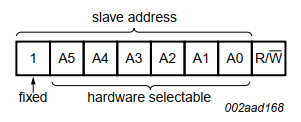
\includegraphics[scale=1]{Chapters/Chapter5/Images/AddressPCA.png}
	\caption{Địa chỉ của module PCA9685}
	\label{fig:C5AddressPCA}
\end{figure}

Các chân A0 tới A5 đều đang thả nổi, địa chỉ của module hiện tại là: 0b1000000 hay 0x40. 

\textbf{Cài đặt xung PWM cho 1 channel:}

Module tính toán thời điểm tắt và bật bằng counter với xung clock đầu vào là 27MHz. Các thanh ghi sử dụng (giả sử đối với channel 0):

LED0\_ON\_H, LED0\_ON\_L: 2 byte này lưu trữ thời điểm IC sẽ xuất tín hiệu ra chân PWM lên mức HIGH.

LED0\_OFF\_H, LED0\_OFF\_L: 2 byte này lưu trữ thời điểm IC sẽ xuất tín hiệu ra chân PWM xuống mức LOW.

Ví dụ cách tính giá trị cần ghi vào các thanh ghi trên:
\begin{align*}
&Delay time =  10\% \\
&PWM Duty Cycle = 20\% (LED on time = 20\%, LED off time = 80\%)
\end{align*}

Tính toán: 
\begin{align*}
Delay time = 4096 \times 10\% = 409.6 \approx 410 = 0x19A
\end{align*}

Do counter đếm từ 0 tới 4096 nên $ Delay time = 0x199 $.
\begin{align*}
&LED0\_ON\_H = 0x1, LED0\_ON\_L = 0x99 \\
&LED \; on \; time = 20\% = 819.2 \sim 819 counts \\
&LED \; off \; time = 0x4CC \\
&LED0\_OFF\_H = 0x4,\; LED0\_OFF\_L = 0xCC 
\end{align*}

\textbf{\textit{Gửi data cho module:}}
\begin{figure}[H]
	\centering
	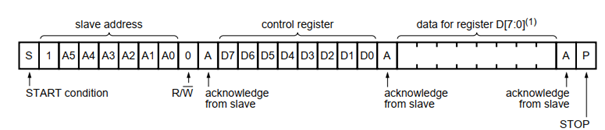
\includegraphics[scale=0.9]{Chapters/Chapter5/Images/SendDataPCA.png}
	\caption{Gửi data cho module PCA9685}
	\label{fig:C5SendDataPCA}
\end{figure}

\begin{lstlisting}
\\ PCA9685_Driver.h
#ifndef PCA9685_H_
#define PCA9685_H_

// include
#include "stm32f4xx_hal.h"

// REGISTER ADDRESSES
#define PCA9685_MODE1       0x00    /**< Mode Register 1 */
#define PCA9685_MODE2       0x01    /**< Mode Register 2 */
#define PCA9685_SUBADR1     0x02    /**< I2C-bus subaddress 1 */
#define PCA9685_SUBADR2     0x03    /**< I2C-bus subaddress 2 */
#define PCA9685_SUBADR3     0x04    /**< I2C-bus subaddress 3 */
#define PCA9685_ALLCALLADR  0x05    /**< LED All Call I2C-bus address */
#define PCA9685_LED0_ON_L   0x06    /**< LED0 on tick, low byte*/
#define PCA9685_LED0_ON_H   0x07    /**< LED0 on tick, high byte*/
#define PCA9685_LED0_OFF_L  0x08    /**< LED0 off tick, low byte */
#define PCA9685_LED0_OFF_H  0x09    /**< LED0 off tick, high byte */

// etc all 16:  LED15_OFF_H 0x45
#define PCA9685_ALLLED_ON_L     0xFA    /**< load all the LEDn_ON registers, low */
#define PCA9685_ALLLED_ON_H     0xFB    /**< load all the LEDn_ON registers, high */
#define PCA9685_ALLLED_OFF_L    0xFC    /**< load all the LEDn_OFF registers, low */
#define PCA9685_ALLLED_OFF_H    0xFD    /**< load all the LEDn_OFF registers,high */
#define PCA9685_PRESCALE        0xFE    /**< Prescaler for PWM output frequency */
#define PCA9685_TESTMODE        0xFF    /**< defines the test mode to be entered */

// MODE1 bits
#define MODE1_ALLCAL    0x01    /**< respond to LED All Call I2C-bus address */
#define MODE1_SUB3      0x02    /**< respond to I2C-bus subaddress 3 */
#define MODE1_SUB2      0x04    /**< respond to I2C-bus subaddress 2 */
#define MODE1_SUB1      0x08    /**< respond to I2C-bus subaddress 1 */
#define MODE1_SLEEP     0x10    /**< Low power mode. Oscillator off */
#define MODE1_AI        0x20    /**< Auto-Increment enabled */
#define MODE1_EXTCLK    0x40    /**< Use EXTCLK pin clock */
#define MODE1_RESTART   0x80    /**< Restart enabled */
// MODE2 bits
#define MODE2_OUTNE_0   0x01    /**< Active LOW output enable input */
#define MODE2_OUTNE_1   0x02    /**< Active LOW output enable input - high impedience */
#define MODE2_OUTDRV    0x04    /**< totem pole structure vs open-drain */
#define MODE2_OCH       0x08  /**< Outputs change on ACK vs STOP */
#define MODE2_INVRT     0x10  /**< Output logic state inverted */

#define PCA9685_I2C_ADDRESS     (0x40<<1)   /**< Default PCA9685 I2C Slave Address */
#define FREQUENCY_OSCILLATOR    25000000    /**< Int. osc. frequency in datasheet */

#define PCA9685_PRESCALE_MIN    3   /**< minimum prescale value */
#define PCA9685_PRESCALE_MAX    255 /**< maximum prescale value */

// Variable
typedef struct PCA9685_Driver {
    I2C_HandleTypeDef *hi2c;
    uint8_t Address;
} PCA9685_HandleTypeDef;

// function
void PCA9685_Init(PCA9685_HandleTypeDef *hpca9685, 
                                    I2C_HandleTypeDef *hi2c,
                                    uint8_t addr,
                                    uint8_t prescale);
void PCA9685_Reset(PCA9685_HandleTypeDef *hpca9685);
void PCA9685_Sleep(PCA9685_HandleTypeDef *hpca9685);
void PCA9685_Wakeup(PCA9685_HandleTypeDef *hpca9685);
void PCA9685_SetExtClk(PCA9685_HandleTypeDef *hpca9685, uint8_t prescale);
void PCA9685_SetPWMFreq(PCA9685_HandleTypeDef *hpca9685, float freq);
uint8_t PCA9685_GetPWM(PCA9685_HandleTypeDef *hpca9685, uint8_t num);
void PCA9685_SetPWM(PCA9685_HandleTypeDef *hpca9685, uint8_t num, uint16_t on, uint16_t off);

void PCA9685_SetOscillatorFrequency(PCA9685_HandleTypeDef *hpca9685, uint32_t freq);

void PCA9685_Write8(PCA9685_HandleTypeDef *hpca9685, uint8_t addr, uint8_t d);
void PCA9685_Read8(PCA9685_HandleTypeDef *hpca9685, uint8_t addr, uint8_t *data);

#endif /* PCA9685_H_ */
\end{lstlisting}

\begin{lstlisting}
\\ PCA9685_Driver.c
/*
*  ======================================================
*            ##### How to use this driver #####
*  ======================================================
*   Set up:
*   #1: Run @ref PCA9685_Init()
*   #2: Run @ref PCA9685_SetOscillatorFrequency(), 27000000
*   #3: Run @ref PCA9685_SetPWMFreq(), 1600
*
*   Let play: @ref PCA9685_SetPWM()
*   #1: GPIO
*   PCA9685_SetPWM(hpca9685, pin, 4096, 0);       // turns pin fully on
*   delay(100);
*   PCA9685_SetPWM(hpca9685, pin, 0, 4096);       // turns pin fully off
*
*   #2: PWM
*   PCA9685_SetPWM(hpca9685, pin, on, off);
*
*
*
 */
#include "PCA9685Driver.h"
uint32_t _oscillator_freq;

void PCA9685_Init(PCA9685_HandleTypeDef *hpca9685, 
                                    I2C_HandleTypeDef *hi2c,
                                    uint8_t addr,
                                    uint8_t prescale) {
    hpca9685->Address = addr;
    hpca9685->hi2c = hi2c;
    PCA9685_Reset(hpca9685);
    if (prescale) {
        PCA9685_SetExtClk(hpca9685, prescale);
    } else {
        // set a default frequency
        PCA9685_SetPWMFreq(hpca9685, 1000);
    }
    // set the default internal frequency
    PCA9685_SetOscillatorFrequency(hpca9685, FREQUENCY_OSCILLATOR);
}
                                    
void PCA9685_Reset(PCA9685_HandleTypeDef *hpca9685) {
    PCA9685_Write8(hpca9685, PCA9685_MODE1, MODE1_RESTART);
    HAL_Delay(10);
}

void PCA9685_Sleep(PCA9685_HandleTypeDef *hpca9685) {
    uint8_t awake;
    PCA9685_Read8(hpca9685, PCA9685_MODE1, &awake);
  uint8_t sleep = awake | MODE1_SLEEP; // set sleep bit high
  PCA9685_Write8(hpca9685, PCA9685_MODE1, sleep);
  HAL_Delay(5); // wait until cycle ends for sleep to be active
}

void PCA9685_Wakeup(PCA9685_HandleTypeDef *hpca9685) {
    uint8_t sleep;
    PCA9685_Read8(hpca9685, PCA9685_MODE1, &sleep);
    uint8_t wakeup = sleep & ~MODE1_SLEEP; // set sleep bit low
    PCA9685_Write8(hpca9685, PCA9685_MODE1, wakeup);
}

void PCA9685_SetExtClk(PCA9685_HandleTypeDef *hpca9685, uint8_t prescale) {
    uint8_t oldmode;
    PCA9685_Read8(hpca9685, PCA9685_MODE1, &oldmode);
    uint8_t newmode = (oldmode & ~MODE1_RESTART) | MODE1_SLEEP; // sleep
    PCA9685_Write8(hpca9685, PCA9685_MODE1, newmode); // go to sleep, turn off internal oscillator
    
    // This sets both the SLEEP and EXTCLK bits of the MODE1 register to switch to
    // use the external clock.
    PCA9685_Write8(hpca9685, PCA9685_MODE1, (newmode |= MODE1_EXTCLK));
    
    PCA9685_Write8(hpca9685, PCA9685_PRESCALE, prescale); // set the prescaler
    
    HAL_Delay(5);
    // clear the SLEEP bit to start
    PCA9685_Write8(hpca9685, PCA9685_MODE1, (newmode & ~MODE1_SLEEP) | MODE1_RESTART | MODE1_AI);
}

void PCA9685_SetPWMFreq(PCA9685_HandleTypeDef *hpca9685, float freq) {
    // Range output modulation frequency is dependant on oscillator
    if (freq < 1)       freq = 1;
    if (freq > 3500)    freq = 3500; // Datasheet limit is 3052=50MHz/(4*4096)

    float prescaleval = ((_oscillator_freq / (freq * 4096.0)) + 0.5) - 1;
    if (prescaleval < PCA9685_PRESCALE_MIN)
    prescaleval = PCA9685_PRESCALE_MIN;
    if (prescaleval > PCA9685_PRESCALE_MAX)
    prescaleval = PCA9685_PRESCALE_MAX;
    uint8_t prescale = (uint8_t)prescaleval;
    
    uint8_t oldmode;
    PCA9685_Read8(hpca9685, PCA9685_MODE1, &oldmode);
    uint8_t newmode = (oldmode & ~MODE1_RESTART) | MODE1_SLEEP; // sleep
    PCA9685_Write8(hpca9685, PCA9685_MODE1, newmode);           // go to sleep
    PCA9685_Write8(hpca9685, PCA9685_PRESCALE, prescale);       // set the prescaler
    PCA9685_Write8(hpca9685, PCA9685_MODE1, oldmode);
    HAL_Delay(5);
    // This sets the MODE1 register to turn on auto increment.
    PCA9685_Write8(hpca9685, PCA9685_MODE1, oldmode | MODE1_RESTART | MODE1_AI);
}

void PCA9685_SetOscillatorFrequency(PCA9685_HandleTypeDef *hpca9685, uint32_t freq) {
    _oscillator_freq = freq;
}

void PCA9685_SetPWM(PCA9685_HandleTypeDef *hpca9685, uint8_t num, uint16_t on, uint16_t off) {
    uint8_t outputBuffer[5] = {PCA9685_LED0_ON_L + 4*num, on, (on >> 8), off, (off >> 8)};
    HAL_I2C_Master_Transmit(hpca9685->hi2c, hpca9685->Address, outputBuffer, 5, 1);
}

            
/******************* Low level I2C interface */
void PCA9685_Write8(PCA9685_HandleTypeDef *hpca9685, uint8_t addr, uint8_t d) {
    HAL_I2C_Mem_Write(hpca9685->hi2c, hpca9685->Address, addr, 1, &d, 1, 1);
}

void PCA9685_Read8(PCA9685_HandleTypeDef *hpca9685, uint8_t addr, uint8_t *data) {
    HAL_I2C_Mem_Read(hpca9685->hi2c, hpca9685->Address, addr, 1, data, 1, 1);
}
\end{lstlisting}

Code điều khiển độ sáng bóng đèn trong file main.c
\begin{lstlisting}
void userPCAInit() {
  PCA9685_Init(&pcaHub, &hi2c2, PCA9685_I2C_ADDRESS, 0);
  PCA9685_SetOscillatorFrequency(&pcaHub, 27000000);
  PCA9685_SetPWMFreq(&pcaHub, 1600);
}

void sendInfoPWM() {
  uint16_t LEDOnTime;
  for (uint8_t channel = 0; channel < 6; channel++) {
    channelON[channel] = DELAY_LED - 1;
    LEDOnTime = intensity[channel / 2] * 4096 / 1000;
    channelOFF[channel]  = (LEDOnTime + DELAY_LED > 4096
                ? LEDOnTime + DELAY_LED - 4096
                : LEDOnTime + DELAY_LED - 1);
    PCA9685_SetPWM(&pcaHub, channel, channelON[channel], channelOFF[channel]);
  }
}
void ControlLED() {
  DecryptData();
  intensity[0] = info[0];
  intensity[1] = info[1];
  intensity[2] = info[2];
  sendInfoPWM();
  HAL_UART_Transmit(&huart2, controlLEDDone, sizeof(controlLEDDone), 10);
  program = IDLE;
}
\end{lstlisting}

\subsection{Nhận tín hiệu từ máy tính và thực hiện các thao tác điều khiển}
Máy tính với VĐK STM32F411VETx đang giao tiếp với nhau bằng UART thông qua IC CP2102.
Để VĐK nhận tín hiệu thì phải quy định trước số byte sẽ gửi, khi nhận đủ số byte này VĐK sẽ chạy hàm ngắt do người dùng định nghĩa. Kích thước gói thông tin nhóm đang quy định là 11 byte theo quy tắc như sau:
\begin{itemize}
\item Kiểm tra giao tiếp UART: \textbf{MT123123123}
\item Đọc giá trị từ cảm biến: \textbf{MG123123123}
\item Điều khiển độ sáng của 3 dàn đèn: \textbf{MLxxxyyyzzz} (xxx, yyy, zzz lần lượt là độ sáng của 3 dàn đèn theo mức độ từ 000 tới 999).
\item Đặt giá trị toạ độ ban đầu của các dàn đèn: \textbf{MIxxxyyyzzz} (xxx, yyy, zzz lần lượt là toạ độ ban đầu của 3 dàn đèn).
\item Gửi giá trị toạ độ mong muốn của các dàn đèn: \textbf{MTxxxyyyzzz} (xxx, yyy, zzz lần lượt là toạ độ mong muốn của 3 dàn đèn).
\end{itemize}

Code nhận tín hiệu trong file main.c:
\begin{lstlisting}
// CHOOSE THE MANUAL CONTROL PROGRAM (It's still under UART interrupt function)
void ManualControl() {
  switch (dataReceived[1]) {
  case 'T':
    program = TEST_UART;
    break;
  case 'I':
    program = SET_INIT_COOR;
    break;
  case 'A':
    program = SET_TARGET_COOR;
    break;
  case 'G':
    program = GET_SENSOR;
    break;
  case 'L':
    program = CONTROL_LED;
    break;
  case 'R':
    program = REINITSENSOR;
    break;
  }
}

// CHOOSE THE AUTO CONTROL PROGRAM (It's still under UART interrupt function)
void AutoControl() {

}

// Select PROGRAM
void HAL_UART_RxCpltCallback(UART_HandleTypeDef *huart)
{
  if (huart->Instance == huart2.Instance) {
    switch (dataReceived[0]) {
    case 'M':
      ManualControl();
      break;
    case 'A':
      AutoControl();
      break;
    }
    HAL_UART_Receive_IT(huart, dataReceived, SIZE_DATA);
  }

}
int main(void)
{
  while (1)
  {
    /* USER CODE END WHILE */

    /* USER CODE BEGIN 3 */
    if (program == TEST_UART) {
      TestUART();
    } else if (program == SET_INIT_COOR) {
      SetInitCoorStepper();
    } else if (program == SET_TARGET_COOR) {
      SetTargetCoorStepper();
    } else if (program == RUN_STEPPER) {
      RunStepper();
    } else if (program == GET_SENSOR) {
      GetSensor();
    } else if (program == CONTROL_LED) {
      ControlLED();
    } else if (program == REINITSENSOR) {
      HAL_UART_Transmit(&huart2, ReInitSensorMessage, sizeof(ReInitSensorMessage), 10);
      userSensorInit();
      program = IDLE;
    }
  }
  /* USER CODE END 3 */
}
\end{lstlisting}


\subsection{Phần mềm điều khiển giao diện trên máy tính}
Có rất nhiều cách để tạo giao diện khác nhau, mỗi ngôn ngữ lập trình như C++, C\#, Python, Java đều cung cấp các thư viện hỗ trợ việc lập trình giao diện. Tuy nhiên nhóm lựa chọn WPF (Windows Presentation Foundation), một hệ thống API hỗ trợ việc xây dựng đồ hoạ trên nền Windows, sử dụng C\# và xaml làm ngôn ngữ lập trình chính. WPF có các ưu điểm sau đây:
\begin{itemize}
\item Mới hơn và do đó phù hợp hơn với các tiêu chuẩn hiện tại.
\item Microsoft đang sử dụng WPF cho rất nhiều ứng dụng mới, ví dụ: Visual Studio.
\item WPF linh hoạt hơn, vì vậy bạn có thể làm nhiều việc hơn mà không phải viết hoặc mua các control mới.
\item Khi bạn cần sử dụng các control của bên thứ 3, các nhà phát triển các control này có thể sẽ tập trung hơn vào WPF vì WPF mới hơn.
\item XAML giúp dễ dàng tạo và chỉnh sửa GUI của bạn và cho phép công việc được phân chia giữa một nhà thiết kế (XAML) và một lập trình viên (C\#, VB.NET, v.v.)
\item Databinding, cho phép bạn có được một sự tách biệt hơn giữa data và layout
\item Sử dụng tăng tốc phần cứng để vẽ GUI, để có hiệu suất tốt hơn
\item WPF cho phép bạn tạo giao diện người dùng cho cả ứng dụng Windows và các ứng dụng web (Silverlight/XBAP)
\end{itemize}
\begin{lstlisting}
\\ MainWindows.xaml
<Window
	xmlns="http://schemas.microsoft.com/winfx/2006/xaml/presentation"
	xmlns:x="http://schemas.microsoft.com/winfx/2006/xaml"
    xmlns:d="http://schemas.microsoft.com/expression/blend/2008" 
    xmlns:mc="http://schemas.openxmlformats.org/markup-compatibility/2006"
    mc:Ignorable="d" x:Class="Serial_Communication_WPF.MainWindow"
    xmlns:ports="clr-namespace:System.IO.Ports;assembly=System"
    Icon="Data Resources\Serial.ico"
    Title="GUI Project" Height="450" Width="504">
    <Window.Resources>
        <ObjectDataProvider ObjectType="{x:Type ports:SerialPort}" MethodName="GetPortNames" x:Key="portNames"/>
        <XmlDataProvider x:Key="ComPorts" Source="CommsData.xml" XPath="/Comms/Ports" />
        <XmlDataProvider x:Key="ComSpeed" Source="CommsData.xml" XPath="/Comms/Baud" />
    </Window.Resources>
    <Grid>
        <Grid.Background>
            <ImageBrush ImageSource="wallpaper.jpg"/>
        </Grid.Background>
        <ComboBox x:Name="cmbComPorts" ItemsSource="{Binding Source={StaticResource portNames}}" SelectionChanged="cmbComPorts_SelectionChanged" HorizontalAlignment="Left" Margin="10,10,0,0" VerticalAlignment="Top" Width="120"/>
        <TextBlock x:Name="tbStatus" HorizontalAlignment="Left" Margin="10,37,0,0" TextWrapping="Wrap" Text="Disconnected" VerticalAlignment="Top" Foreground="Red"/>
        <Button x:Name="btnConnect" Content="Connect" HorizontalAlignment="Left" Margin="135,10,0,0" VerticalAlignment="Top" Width="75" Click="btnConnect_Click"/>
        <TabControl HorizontalAlignment="Left" Margin="10,58,0,10" Width="476" Background="{x:Null}">
            <TabItem x:Name="tabManual" Header="Manual">
                <Grid>
                    <Grid.Background>
                        <SolidColorBrush Color="Black" Opacity="0.4"/>
                    </Grid.Background>
                    <Button x:Name="btnTestUART" Content="Test UART" HorizontalAlignment="Left" Margin="347,35,0,0" VerticalAlignment="Top" Width="111" Click="btnTestUART_Click" Height="30"/>
                    <RichTextBox x:Name="Commdata" HorizontalAlignment="Left" Height="108" Margin="10,35,0,0" VerticalAlignment="Top" Width="316">
                        <FlowDocument>
                            <Paragraph>
                                <Run Text=""/>
                            </Paragraph>
                        </FlowDocument>
                    </RichTextBox>

                    <Button x:Name="btnGetSensors" Content="Get Sensors Data" HorizontalAlignment="Left" Margin="347,70,0,0" VerticalAlignment="Top" Width="111" Height="30" Click="btnGetSensors_Click"/>
                    <TextBlock x:Name="tbTerminal" HorizontalAlignment="Center" Margin="130,10,247,0" TextWrapping="Wrap" Text="Data Received" VerticalAlignment="Top" Height="20" Foreground="White"/>
                    <Slider x:Name="slLevelLamp0" HorizontalAlignment="Left" Margin="144,148,0,0" VerticalAlignment="Top" Width="316" Maximum="999" TickFrequency="10" TickPlacement="BottomRight" IsSnapToTickEnabled="True" ValueChanged="slLevelLamp0_ValueChanged" PreviewMouseUp="slLevelLamp_PreviewMouseUp"/>
                    <Slider x:Name="slLevelLamp1" HorizontalAlignment="Left" Margin="144,177,0,0" VerticalAlignment="Top" Width="316" Maximum="999" TickFrequency="10" TickPlacement="BottomRight" IsSnapToTickEnabled="True" ValueChanged="slLevelLamp1_ValueChanged" PreviewMouseUp="slLevelLamp_PreviewMouseUp"/>
                    <Slider x:Name="slLevelLamp2" HorizontalAlignment="Left" Margin="144,206,0,0" VerticalAlignment="Top" Width="316" Maximum="999" TickFrequency="10" TickPlacement="BottomRight" IsSnapToTickEnabled="True" ValueChanged="slLevelLamp2_ValueChanged" PreviewMouseUp="slLevelLamp_PreviewMouseUp"/>

                    <TextBlock x:Name="tbLevelLamp0" HorizontalAlignment="Left" Margin="10,149,0,0" TextWrapping="Wrap" Text="Level Lamp 0" VerticalAlignment="Top" Height="18" Foreground="White"/>
                    <TextBlock x:Name="tbLevelLamp1" HorizontalAlignment="Left" Margin="10,178,0,0" TextWrapping="Wrap" Text="Level Lamp 1" VerticalAlignment="Top" Height="18" Foreground="White"/>
                    <TextBlock x:Name="tbLevelLamp2" HorizontalAlignment="Left" Margin="10,207,0,0" TextWrapping="Wrap" Text="Level Lamp 2" VerticalAlignment="Top" Height="18" Foreground="White"/>
                    <TextBox x:Name="txtValueL0" HorizontalAlignment="Left" Height="19" Margin="84,148,0,0" TextWrapping="Wrap" Text="0" VerticalAlignment="Top" Width="55"/>
                    <TextBox x:Name="txtValueL1" HorizontalAlignment="Left" Height="19" Margin="84,177,0,0" TextWrapping="Wrap" Text="0" VerticalAlignment="Top" Width="55"/>
                    <TextBox x:Name="txtValueL2" HorizontalAlignment="Left" Height="19" Margin="84,206,0,0" TextWrapping="Wrap" Text="0" VerticalAlignment="Top" Width="55"/>
                    <TextBlock x:Name="tbStepper" HorizontalAlignment="Left" Margin="109,235,0,0" TextWrapping="Wrap" Text="Location of Light-Beams" VerticalAlignment="Top" Foreground="White"/>
                    <TextBox x:Name="txtLocStep0" HorizontalAlignment="Left" Height="23" Margin="10,280,0,0" TextWrapping="Wrap" Text="0" VerticalAlignment="Top" Width="57" PreviewTextInput="txtLocStep_PreviewTextInput"/>
                    <TextBox x:Name="txtLocStep1" HorizontalAlignment="Left" Height="23" Margin="78,280,0,0" TextWrapping="Wrap" Text="0" VerticalAlignment="Top" Width="57" PreviewTextInput="txtLocStep_PreviewTextInput"/>
                    <TextBox x:Name="txtLocStep2" HorizontalAlignment="Left" Height="23" Margin="144,280,0,0" TextWrapping="Wrap" Text="0" VerticalAlignment="Top" Width="57" PreviewTextInput="txtLocStep_PreviewTextInput"/>
                    <TextBlock x:Name="tbBeam0" HorizontalAlignment="Left" Margin="18,260,0,0" TextWrapping="Wrap" Text="Beam 0" VerticalAlignment="Top" Width="40" Height="16" Foreground="White"/>
                    <TextBlock x:Name="tbBeam1" HorizontalAlignment="Left" Margin="86,260,0,0" TextWrapping="Wrap" Text="Beam 1" VerticalAlignment="Top" Width="40" Height="16" Foreground="White"/>
                    <TextBlock x:Name="tbBeam2" HorizontalAlignment="Left" Margin="153,260,0,0" TextWrapping="Wrap" Text="Beam 2" VerticalAlignment="Top" Width="40" Height="16" Foreground="White"/>
                    <Button x:Name="btnSetTarget" Content="Set Target Location" HorizontalAlignment="Left" Margin="211,280,0,0" VerticalAlignment="Top" Width="115" Height="23" Click="btnSetTarget_Click"/>
                    <Button x:Name="btnSetCurrent" Content="Set Current Location" HorizontalAlignment="Left" Margin="332,280,0,0" VerticalAlignment="Top" Width="126" Height="23" Click="btnSetCurrent_Click"/>
                    <Button x:Name="btnReInitSensor" Content="Reset Sensors" HorizontalAlignment="Left" Margin="347,105,0,0" VerticalAlignment="Top" Width="111" Height="30" Click="btnReInitSensor_Click"/>
                </Grid>
            </TabItem>
            <TabItem x:Name="tabAuto" Header="Auto">
                <Grid Background="#FFE5E5E5">
                    <Grid.ColumnDefinitions>
                        <ColumnDefinition Width="5*"/>
                        <ColumnDefinition Width="108*"/>
                    </Grid.ColumnDefinitions>
                </Grid>
            </TabItem>
        </TabControl>
    </Grid>
</Window>
\end{lstlisting}

\begin{lstlisting}
\\ MainWindows.xaml.cs
using System;
using System.Collections.Generic;
using System.Linq;
using System.Text;
using System.Windows;
using System.Windows.Controls;
using System.Windows.Data;
using System.Windows.Documents;
using System.Windows.Input;
using System.Windows.Media;
using System.Windows.Media.Imaging;
using System.Windows.Navigation;
using System.Windows.Shapes;
using System.IO.Ports;
using System.Threading;
using System.Windows.Threading;
using System.Text.RegularExpressions;

namespace Serial_Communication_WPF
{
    /// <summary>
    /// Interaction logic for MainWindow.xaml
    /// </summary>
    public partial class MainWindow : Window
    {
        #region variables
        //Richtextbox
        FlowDocument mcFlowDoc = new FlowDocument();
        Paragraph para = new Paragraph();
        //Serial 
        SerialPort serial = new SerialPort();
        string recieved_data;
        Boolean flagConnect = false;
        // level LAMP
        int levelLamp0;
        int levelLamp1;
        int levelLamp2;
        #endregion

        #region MainWindow and UART Function
        public MainWindow()
        {
            InitializeComponent();
            
        }
        private void cmbComPorts_SelectionChanged(object sender, SelectionChangedEventArgs e)
        {
            var selectedComboItem = sender as ComboBox;
            string name = selectedComboItem.SelectedItem as string;
        }
        private void btnConnect_Click(object sender, RoutedEventArgs e)
        {
            if (flagConnect == false)
            {
                //Sets up serial port
                string portName = cmbComPorts.SelectedValue as string;
                serial.PortName = portName;
                serial.BaudRate = 115200;
                serial.Handshake = System.IO.Ports.Handshake.None;
                serial.Parity = Parity.None;
                serial.DataBits = 8;
                serial.StopBits = StopBits.Two;
                serial.ReadTimeout = 200;
                serial.WriteTimeout = 50;
                serial.Open();
                flagConnect = true;

                //Sets button State and Creates function call on data recieved
                btnConnect.Content = "Disconnect";
                this.tbStatus.Text = "Connected!";
                this.tbStatus.Foreground = new SolidColorBrush(Colors.Green);
                serial.DataReceived += new System.IO.Ports.SerialDataReceivedEventHandler(Recieve);

            }
            else
            {
                try // just in case serial port is not open could also be acheved using if(serial.IsOpen)
                {
                    serial.Close();
                    btnConnect.Content = "Connect";
                    this.tbStatus.Text = "Disconnected!";
                    this.tbStatus.Foreground = new SolidColorBrush(Colors.Red);
                    flagConnect = false;
                }
                catch
                {
                }
            }
        }
        #endregion

        #region Recieving

        private delegate void UpdateUiTextDelegate(string text);
        private void Recieve(object sender, System.IO.Ports.SerialDataReceivedEventArgs e)
        {
            // Collecting the characters received to our 'buffer' (string).
            recieved_data = serial.ReadExisting(); 
            Dispatcher.Invoke(DispatcherPriority.Send, new UpdateUiTextDelegate(WriteData), recieved_data);
        }
        private void WriteData(string text)
        {
            // Assign the value of the recieved_data to the RichTextBox.
            para.Inlines.Add(text);
            mcFlowDoc.Blocks.Add(para);
            Commdata.Document = mcFlowDoc;
            Commdata.ScrollToEnd();
        }

        #endregion

        #region Sending with Button    
        private void btnTestUART_Click(object sender, RoutedEventArgs e)
        {
            SerialCmdSend("MT123123123");
        }
        private void btnGetSensors_Click(object sender, RoutedEventArgs e)
        {
            SerialCmdSend("MG123123123");
        }
        public void SerialCmdSend(string data)
        {
            if (serial.IsOpen)
            {
                try
                {
                    // Send the binary data out the port
                    byte[] hexstring = Encoding.ASCII.GetBytes(data);
                    //There is a intermitant problem that I came across
                    //If I write more than one byte in succesion without a 
                    //delay the PIC i'm communicating with will Crash
                    //I expect this id due to PC timing issues ad they are
                    //not directley connected to the COM port the solution
                    //Is a ver small 1 millisecound delay between chracters
                    foreach (byte hexval in hexstring)
                    {
                        byte[] _hexval = new byte[] { hexval }; // need to convert byte to byte[] to write
                        serial.Write(_hexval, 0, 1);
                        Thread.Sleep(1);
                    }
                }
                catch (Exception)
                {
                    //para.Inlines.Add("Failed to SEND" + data + "\n" + ex + "\n");
                    //mcFlowDoc.Blocks.Add(para);
                    //Commdata.Document = mcFlowDoc;
                }
            }
            else
            {
            }
        }

        #endregion

        #region Form Controls

        private void Close_Form(object sender, RoutedEventArgs e)
        {
            if (serial.IsOpen) serial.Close();
            this.Close();
        }
        private void Max_size(object sender, RoutedEventArgs e)
        {
            if (this.WindowState != WindowState.Maximized) this.WindowState = WindowState.Maximized;
            else this.WindowState = WindowState.Normal;
        }
        private void Min_size(object sender, RoutedEventArgs e)
        {
            if (this.WindowState != WindowState.Minimized) this.WindowState = WindowState.Minimized;
            else this.WindowState = WindowState.Normal;
        }
        private void Move_Window(object sender, MouseButtonEventArgs e)
        {
            this.DragMove();
        }
        #endregion

        #region Lights Level
        private void slLevelLamp0_ValueChanged(object sender, RoutedPropertyChangedEventArgs<double> e)
        {
            var slide = sender as Slider;
            txtValueL0.Text = slide.Value.ToString();
        }
        private void slLevelLamp1_ValueChanged(object sender, RoutedPropertyChangedEventArgs<double> e)
        {
            var slide = sender as Slider;
            txtValueL1.Text = slide.Value.ToString();
        }

        private void slLevelLamp2_ValueChanged(object sender, RoutedPropertyChangedEventArgs<double> e)
        {
            var slide = sender as Slider;
            txtValueL2.Text = slide.Value.ToString();
        }

        private void slLevelLamp_PreviewMouseUp(object sender, MouseButtonEventArgs e)
        {
            var slide = sender as Slider;
            if (slide.Name == "slLevelLamp0") 
            {
                levelLamp0 = Convert.ToInt16(slide.Value);
            }
            else if (slide.Name == "slLevelLamp1")
            {
                levelLamp1 = Convert.ToInt16(slide.Value);
            }
            else if (slide.Name == "slLevelLamp2")
            {
                levelLamp2 = Convert.ToInt16(slide.Value);
            }
            char[] lightMessage = new char[11];
            lightMessage[0] = 'M';
            lightMessage[1] = 'L';
            // Level Lamp0
            lightMessage[4] = (char)((levelLamp0 % 10) + 48);
            lightMessage[3] = (char)((levelLamp0 / 10 % 10) + 48);
            lightMessage[2] = (char)((levelLamp0 / 100 % 10) + 48);
            // Level Lamp1
            lightMessage[7] = (char)((levelLamp1 % 10) + 48);
            lightMessage[6] = (char)((levelLamp1 / 10 % 10) + 48);
            lightMessage[5] = (char)((levelLamp1 / 100 % 10) + 48);
            // Level Lamp2
            lightMessage[10] = (char)((levelLamp2 % 10) + 48);
            lightMessage[9] = (char)((levelLamp2 / 10 % 10) + 48);
            lightMessage[8] = (char)((levelLamp2 / 100 % 10) + 48);
            string s = new string(lightMessage);
            //WriteData(s);
            SerialCmdSend(s);
        }
        private void btnReInitSensor_Click(object sender, RoutedEventArgs e)
        {
            SerialCmdSend("MR123123123");
        }
        #endregion

        #region Stepper
        private void btnSetTarget_Click(object sender, RoutedEventArgs e)
        {
            char[] TargetMessage = new char[11];
            int tarStep0, tarStep1, tarStep2;
            Int32.TryParse(txtLocStep0.Text, out tarStep0);
            Int32.TryParse(txtLocStep1.Text, out tarStep1);
            Int32.TryParse(txtLocStep2.Text, out tarStep2);

            TargetMessage[0] = 'M';
            TargetMessage[1] = 'A';
            // Level Lamp0
            TargetMessage[4] = (char)((tarStep0 % 10) + 48);
            TargetMessage[3] = (char)((tarStep0 / 10 % 10) + 48);
            TargetMessage[2] = (char)((tarStep0 / 100 % 10) + 48);
            // Level Lamp1
            TargetMessage[7] = (char)((tarStep1 % 10) + 48);
            TargetMessage[6] = (char)((tarStep1 / 10 % 10) + 48);
            TargetMessage[5] = (char)((tarStep1 / 100 % 10) + 48);
            // Level Lamp2
            TargetMessage[10] = (char)((tarStep2 % 10) + 48);
            TargetMessage[9] = (char)((tarStep2 / 10 % 10) + 48);
            TargetMessage[8] = (char)((tarStep2 / 100 % 10) + 48);
            string s = new string(TargetMessage);
            SerialCmdSend(s);
        }

        private void btnSetCurrent_Click(object sender, RoutedEventArgs e)
        {
            char[] CurrentMessage = new char[11];
            int curStep0, curStep1, curStep2;
            Int32.TryParse(txtLocStep0.Text, out curStep0);
            Int32.TryParse(txtLocStep1.Text, out curStep1);
            Int32.TryParse(txtLocStep2.Text, out curStep2);
            CurrentMessage[0] = 'M';
            CurrentMessage[1] = 'I';
            // Level Lamp0
            CurrentMessage[4] = (char)((curStep0 % 10) + 48);
            CurrentMessage[3] = (char)((curStep0 / 10 % 10) + 48);
            CurrentMessage[2] = (char)((curStep0 / 100 % 10) + 48);
            // Level Lamp1
            CurrentMessage[7] = (char)((curStep1 % 10) + 48);
            CurrentMessage[6] = (char)((curStep1 / 10 % 10) + 48);
            CurrentMessage[5] = (char)((curStep1 / 100 % 10) + 48);
            // Level Lamp2
            CurrentMessage[10] = (char)((curStep2 % 10) + 48);
            CurrentMessage[9] = (char)((curStep2 / 10 % 10) + 48);
            CurrentMessage[8] = (char)((curStep2 / 100 % 10) + 48);
            string s = new string(CurrentMessage);
            SerialCmdSend(s);
        }
        private void txtLocStep_PreviewTextInput(object sender, TextCompositionEventArgs e)
        {
            Regex regex = new Regex("[^0-9]+");
            e.Handled = regex.IsMatch(e.Text);
        }

        #endregion
    }
}
\end{lstlisting}

Giao diện của ứng dụng điều khiển (Hình~\ref{fig:C5GUI}):
\begin{figure}[ht]
	\centering
	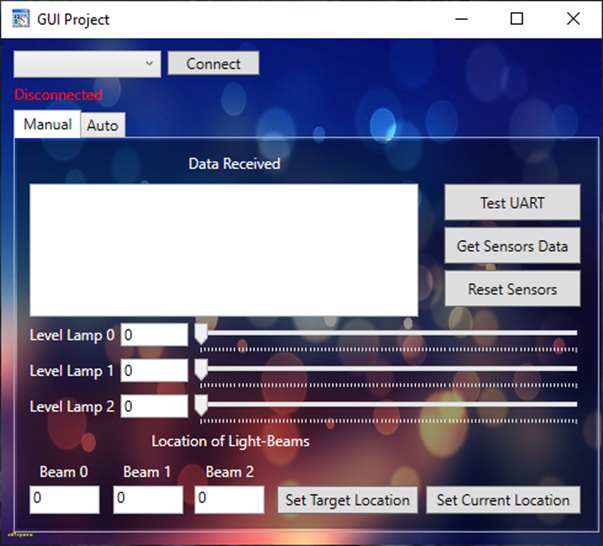
\includegraphics[scale=0.9]{Chapters/Chapter5/Images/GUI.png}
	\caption{Giao diện GUI của ứng dụng điều khiển}
	\label{fig:C5GUI}
\end{figure}

Các trình điều khiển có trên giao diện:
\begin{itemize}
\item Combobox chọn port kết nối với module UART CP2102. Nút nhấn Connect để kết nối với port đã chọn. Có textblock hiển thị trạng thái kết nối.
\item Textbox “Data received” để nhận dữ liệu từ VĐK và hiển thị lên màn hình.
\item Nút nhấn TestUART để kiểm tra kết nối UART có ổn định hay không. Nếu ổn định thì trên textbox “Data Received” sẽ hiển thị dòng chữ: "Welcome to Project: Automatic light intensity balance".
\item Nút GetSensors Data để gửi lệnh đọc cảm biến. Dữ liệu trả về sẽ hiển thị lên textbox.
\item Nút Reset Sensors để gửi lệnh reset và khởi tạo lại các cảm biến trong trường hợp dữ liệu trả về bị sai sót, không chính xác.
\item 3 Slide Level Lamp để điều chỉnh độ sáng của 3 thanh dàn đèn.
\item Nút Set Current Location để gửi toạ độ ban đầu của các thanh dàn đèn.
\item Nút Set Target Location để gửi toạ độ mong muốn cho các thanh dàn đèn. 
\end{itemize}
